%  !TeX  root  =  user_guide.tex

\section{Extension SQL Anywhere}\label{sec:sqlanywhere}

% when the revision of a section has been finalized, 
% comment out the following line:
% \updatedisclaimer

SQL Anywhere est un système de gestion de base de données relationnel propriétaire (SGBDR) édité par Sybase. SQL Anywhere inclu la gestion spatiale selon les standards de l'OGC et des fonctions internes pour exporter dans les formats KML, GML et SVG.

L'extension \toolbtntwo{sqlanywhere}{SQL Anywhere} fournie un pilote de données natif à QGIS sous la licence GPL v3.  L'extension permet 
de se connecter à une base SQL Anywhere. La boîte de dialogue \dialog{Ajouter une couche SQL Anywhere} est similaire dans ses fonctionnalités à celle pour PostGIS et SpatiaLite.

\begin{figure}[ht]
   \centering
   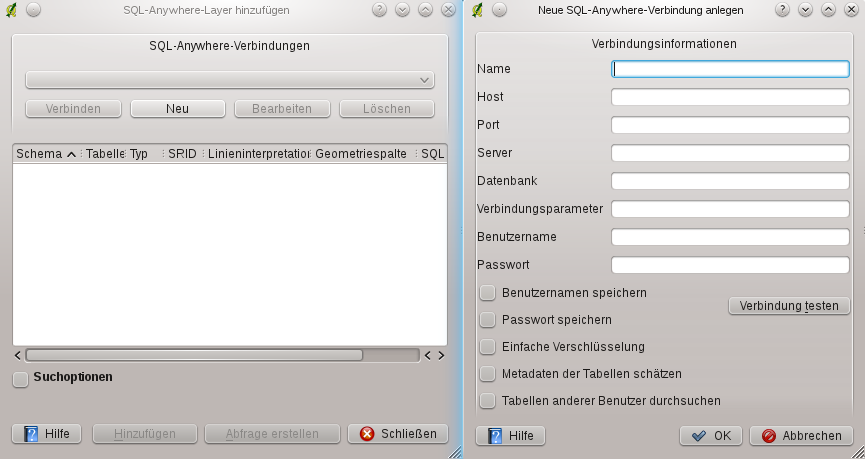
\includegraphics[clip=true, width=14cm]{sql_anywhere}
   \caption{Boîte de dialogue SQL Anywhere \nixcaption}
   \label{fig:sqlanywhere}
\end{figure}

\FloatBarrier